\documentclass[12pt, a4paper]{book}
\begin{document}

Now is the time to focus on the critical task of preparing the data for our DM search using ML. This task is essential because accurately distinguishing between signal and background events is a key challenge in searching for any new signal event, 
as seen in Chapter \ref{sec:data_anal}. In this chapter we will define what \textit{background} and \textit{signal} actually are, as well as selecting appropriate kinematical cuts to define the preselection region for our search. In addition, we will 
explain the data preparing procedure such that it is in a format that is well-suited for our ML algorithms. The reason this process is of great importance is, so we can maximize the chances of our ML algorithm to accurately identify any DM signals. 
Moreover, by providing a detailed explanation of the data preparation process, we can ensure that our dataset is both reliable and effective, and that our analysis is robust and trustworthy. In short, this chapter represents a critical step towards 
achieving our goal of using ML to classify DM from SM events using ATLAS data, and it is essential to the success of our overall research goal.



\clearpage
\section{Standard Model background estimation}\label{sec:SM_bkgs}
As we are going to look at dilepton final states with missing transverse energy to try to teach our ML to learn DM signatures, then we need to take into account all possible SM background event that have this kind of final states. The SM backgrounds processes we will look at are explained in the next subsections. 
In Appendix \ref{appendix:DSIDs} is the full list of dataset IDs for background process used in this thesis.

\subsection{W and Drell Yan}
$W$+jets and $Z/\gamma^*$+jets can decay into final states that mimic the one we are searching for. The $W$ boson can give us a lepton and neutrino $W\rightarrow l\nu_l$, which gives us MET, and $Z/\gamma\rightarrow ll$, which gives us a dilepton final state. 
The dominant production mechanism for these background processes be seen in Figure \ref{fig:WZG_BKG}. As the $W$ boson behaves differently than the $Z$ and $\gamma$, as the $W$ boson can decay into neutrinos giving us MET. 
We will divide these background processes into two, $W$ and \textit{Drell Yan} processes, where the latter is $Z/\gamma^*$ + jets. To simulate these background processes Sherpa 2.2.11 \cite{Sherpa} was used.
\graphicspath{{../../figures/}}
\begin{figure}[!ht]
    \centering
    \includegraphics[width=\textwidth]{WZGjetsBKG.png}
    \caption[$W$ and Drell Yan production]{Diagrams showcasing SM $W$ and Drell Yan production. A quark marked with a prime, indicated that the quark might be a different flavor after interacting with a boson.}\label{fig:WZG_BKG}
\end{figure}

\subsection{Top pair}
Another SM background process we will look at are processes that have a $t\bar{t}$ in them. Since the top has a close to 100\% branching ratio of decaying into a $b$-quark\footnote{Making $b-$tagging an effective method to isolate this background channel} and a $W$ boson, $t\rightarrow bW^+$, where the $W$ boson can again decay into a neutrino and lepton,
where the first gives us MET. The main production mechanism for these processes can be seen in Figure \ref{fig:TT_BKG}. To simulate these background processes Powheg-Box v2 \cite{PowHeg} interfaced with Pythia 8 \cite{Pythia} was used.
\begin{figure}[!ht]
    \centering
    \begin{subfigure}[b]{0.3\textwidth}
        \centering
        \includegraphics[width=\textwidth]{TTBar1.png}
        \caption{$s$-channel}
    \end{subfigure}
    \hfill
    \begin{subfigure}[b]{0.3\textwidth}
        \centering
        \includegraphics[width=0.9\textwidth]{TTBar2.png}
        \caption{Gluon fusion}
    \end{subfigure}
    \hfill
    \begin{subfigure}[b]{0.3\textwidth}
        \centering
        \includegraphics[width=\textwidth]{TTBar3.png}
        \caption{$t$-channel}
    \end{subfigure}
    \caption[$t\bar{t}$ production]{Diagrams showcasing SM $t\bar{t}$ production}\label{fig:TT_BKG}
\end{figure}

\subsection{Single top}
On the same note we have processes with a single top. Where again the top has a high branching ratio of decaying into a $b$-quark and a $W$ boson, $t\rightarrow bW^+$, where the $W$ boson can again decay into a neutrino giving 
us MET. The main production mechanism for these processes can be seen in Figure \ref{fig:T_BKG}. To simulate these background processes Powheg-Box v2 \cite{PowHeg} interfaced with Pythia 8 \cite{Pythia} was used.
\begin{figure}[!ht]
    \centering
    \begin{subfigure}[b]{0.3\textwidth}
        \centering
        \includegraphics[width=\textwidth]{SingleTop1.png}
        \caption{$s$-channel}
    \end{subfigure}
    \hfill
    \begin{subfigure}[b]{0.3\textwidth}
        \centering
        \includegraphics[width=\textwidth]{SingleTop2.png}
        \caption{$t$-channel}
    \end{subfigure}
    \hfill
    \begin{subfigure}[b]{0.3\textwidth}
        \centering
        \includegraphics[width=\textwidth]{SingleTop3.png}
        \caption{$tW$}
    \end{subfigure}
    \caption[Single Top production]{Diagrams showcasing SM single top productions.  A quark marked with a prime, indicated that the quark might be a different flavor after interacting with a boson.}\label{fig:T_BKG}
\end{figure}

\subsection{Diboson}
The last SM background process we will look at are processes containing two bosons, called \textit{diboson} backgrounds. The two SM bosons we will consider when looking into these final states are the $W$ and $Z$, as these can decay as $Z\rightarrow ll$ 
or $W\rightarrow l\nu_l$, where the prime means a different lepton flavor. The main production mechanism for these processes can be seen in Figure \ref{fig:Diboson_BKG}. To simulate these background processes Sherpa 2.2.11 \cite{Sherpa} was used.
\begin{figure}[!ht]
    \centering 
    \begin{subfigure}[b]{0.4\textwidth}
        \centering
        \includegraphics[width=\textwidth]{Diboson1.png}
        \caption{$s$-channel $WZ$}
    \end{subfigure}
    \hfill
    \begin{subfigure}[b]{0.4\textwidth}
        \centering
        \includegraphics[width=\textwidth]{Diboson2.png}
        \caption{$s$-channel $WW$}
    \end{subfigure}
    \hfill
    \begin{subfigure}[b]{0.4\textwidth}
        \centering
        \includegraphics[width=\textwidth]{Diboson3.png}
        \caption{$t$-channel $WZ$}
    \end{subfigure}
    \hfill
    \begin{subfigure}[b]{0.4\textwidth}
        \centering
        \includegraphics[width=\textwidth]{Diboson4.png}
        \caption{$t$-channel $WW$ and $ZZ$}
    \end{subfigure}
    \caption[Diboson production]{Diagrams showcasing SM diboson production. A star superscript on a boson indicates that the boson needs to be virtual and off mass shell.  A quark marked with a prime, indicated that the quark might be a different flavor after interacting with a boson. }\label{fig:Diboson_BKG}
\end{figure}

\section{Dark Matter samples}\label{chap:DM_sample}
\subsection{Mono-Z'}
The models in Chapter \ref{chap:DM} contain three relevant couplings
\begin{itemize}
    \item the coupling $g_D$ between the $Z'$ and the DM particles ($Z'Z'h_D$ or $Z'\chi_1\chi_2$)
    \item the coupling $g_q$ between the $Z'$ and quarks
    \item and the coupling $g_l$ between the $Z'$ and leptons
\end{itemize}
The coupling to quarks and leptons are assumed to be the same for all generations. When simulating the couplings were set to
\begin{itemize}
    \item $g_D = 1$,
    \item $g_q=0.1$,
    \item and $g_l=0.01$.
\end{itemize}
In addition to the couplings, as mentioned on Chapter \ref{chap:DM}, we will divide the three models, DH, LV and EFT into two more regions. The difference being the masses, Table \ref{tab:DMass} showcases the definition of the Light Dark Sector (LDS) and Heavy Dark Sector (HDS).
\begin{table}[!h]
    \centering\caption{Dark sector masses in light- and heavy dark sector models}
    \begin{tabular}{l|c|c}\midrule\midrule
                                                                            & Dark Higgs            & Light Vector / Inelastic EFT              \\\midrule
        \multirow{2}{*}[-2\baselineskip]{Light Dark Sector}                 & $m_\chi = 5$ GeV      & $m_{\chi_1}= 5$ GeV                       \\
                                                                            & $m_{h_D} = 125$ GeV   & $m_{\chi_2}= m_{\chi_1}+m_{Z'} + 25$ GeV  \\\midrule
        \multirow{2}{*}[-2\baselineskip]{Heavy Dark Sector}                 & $m_\chi = 5$ GeV      & $m_{\chi_1}= m_{Z'}/2$                    \\
                                                                            & $m_{h_D} = m_{Z'}$    & $m_{\chi_2}= 2m_{Z'}$                     \\\midrule\midrule
    \end{tabular}
    \label{tab:DMass}
\end{table}
\newpage\noindent The simulated masses of the new $Z'$ boson for this thesis are
$$
m_{Z'} = [130, 200, 400, 600, 800, 900, 1100, 1200, 1300, 1400, 1500]\text{ GeV},
$$
for the DH and LV model and 
$$
m_{Z'} = [130, 200, 300, 400, 500, 600, 700, 800, 900, 1000, 1100, 1200, 1300, 1400, 1500]\text{ GeV},
$$
or the EFT model.
\subsection{Supersymmetric direct slepton production}
For the supersymmetric direct slepton production model, $\tilde{\ell}\tilde{\ell}\rightarrow \ell\ell\tilde{\chi}_1^0\tilde{\chi}_1^0$, the masses of the sleptons, $m_{\tilde{\ell}}$, and neutralinos, $m_{\tilde{\chi}_1^0}$ are the parameters that will be changed. 
The masses used in this thesis are shown below 
$$
m_{\tilde{\ell}} = [90, 100, 125, 150, 175, 200, 225, 250, 275, 300, 350, 400]\text{ GeV},
$$
and
$$
m_{\tilde{\chi}_1^0} = [1, 25, 30, 40, 50, 60, 70, 75, 80, 85, 90, 95, 100, 105, 110, 120, 125,
$$
$$
130, 135, 140, 145, 150, 155,
160, 170, 175, 180, 185, 195, 200, 205
$$
$$
210, 220, 230, 235,
 245, 250, 255, 260, 270, 280, 300, 330, 350, 380 ]\text{ GeV}
$$
\subsection{2HDM + a}
For the Two Higgs Doublet Model with an additional pseudoscalar $a$ which decays into DM there are three important parameters, the mass of the new charged Higgs, which we will call $m_{H^-}$. The mass of the pseudoscalar $a$, $m_a$ and ratio between the vacuum expectation values of the Higgs doublet, $\tan\beta$. The values used for this thesis can be sen below.
$$
m_{H^-} = [300, 400, 500, 600, 700, 800, 900, 1000, 1200, 
$$
$$
1250, 1300, 1500, 1600, 1700, 1800, 2000, 2100]\text{ GeV},
$$
and 
$$
m_a = [100, 150, 200, 250, 300, 350, 400, 450, 500, 600, 700, 800]\text{ GeV},
$$
and 
$$
\tan\beta = [1, 5, 10, 20, 30]
$$
In this thesis we assume the DM candidate mass of this model to be $m_{\chi}=10$ GeV. 
\section{Object selection}\label{sec:obj_sel}
Before getting into our DM search and the regions we will study we have to define how standard objects are defined. By standard objects we mean electrons, muons and jets. As this thesis is made using ATLAS data and simulations we will be following the central recommendations.%\\
% \\The electrons \todo{I don't know how else to present these}are selected using the criteria on Table \ref{tab:E_selec}. The muons are selected using the criteria on Table \ref{tab:mu_selec}. The jets are selected using the criteria on Table \ref{tab:jet_selec}. The missing transverse energy is reconstructed from jets selected and calibrated according to the information in Table \ref{tab:jet_selec}. In addition to these a kinematical cut of $m_{ll}>10$ GeV will be made to exclude hadron productions.
% \begin{table}[!h]
%     \centering\caption[Electron selection criteria]{Electron selection criteria.}
%     \begin{tabular}{l|r}\midrule\midrule
%         Feature                                                                 & Selection criteria        \\\midrule
%         Transverse momentum                                                     & $p_T > 25$ GeV     \\
%         Pseudorapidity range                                                    & $\abs{\eta}<1.37$ or  $1.52<\abs{\eta}<2.47$ \\
%         $d_0$ significance cut                                                  & $\abs{d_0(\sigma)}<5$    \\
%         $z_0$ cut                                                               & $\abs{\Delta z_0\sin\theta}<0.5$mm    \\\midrule\midrule
%     \end{tabular}
%     \label{tab:E_selec}
% \end{table}
% \begin{table}[!h]
%     \centering\caption[Muon selection criteria]{Muon selection criteria.}
%     \begin{tabular}{l|r}\midrule\midrule
%         Feature                                                                 & Selection criteria        \\\midrule
%         Transverse momentum                                                      & $p_T > 27(20)$ GeV for leading (sub-leading)     \\
%         Pseudorapidity cut                                                      & $\abs{\eta}<2.5$ \\
%         $d_0$ significance cut                                                  & $\abs{d_0(\sigma)}<5$    \\
%         $z_0$ cut                                                               & $\abs{\Delta z_0\sin\theta}<0.5$mm    \\\midrule\midrule
%     \end{tabular}
%     \label{tab:mu_selec}
% \end{table}
% \begin{table}[!h]
%     \centering\caption[Jet selection criteria]{Jet selection criteria.}
%     \begin{tabular}{l|r}\midrule\midrule
%         Feature                                                                 & Selection criteria        \\\midrule
%         Algorithm                                                               & Anti-$k_t$     \\
%         $R$-parameter                                                           & 0.4     \\\midrule
%         Transverse momentum                                                     & $p_T > 20$ GeV     \\
%         Pseudorapidity cut                                                      & $\abs{\eta}<4.5$ \\
%         Jet Vertex Tagger                                                       & $>0.5$ for $p_T<60$ GeV, $\abs{\eta}<2.4$ \\
%         forward JVT                                                             & fJVT $<0.4$ and |timing| < 10 ns for $p_T<120$ GeV, $2.5<\abs{\eta}<4.5$ \\\midrule
%         b-jet tagging                                                           & DL1r score > 0.665 with 85\% efficiency \\\midrule\midrule
%     \end{tabular}
%     \label{tab:jet_selec}
% \end{table}



\section{Preselection region}
Now that we have defined what our backgrounds and signals are, the next step is to create a so-called \textit{preselection region}. The preselection region is the kinematical region we will use as a base for our search. As we are conducting a model independent search we want 
our kinematical cuts to be minimal and as general as possible. As we are looking at a dilepton final state, then we need to first define what we mean by that. If we were only searching for DM with the $Z'$ model, then a sensible definition would be 
Same Flavor Opposite Sign (SFOS) leptons ($e^\pm e^\mp, \mu^\pm\mu^\mp$). However, to stay as general, and model independent, as possible we will also study other possible combinations as these might be important for theories such as SUSY or Lepton Flavor Violating 
(LFV) models. These are Different Flavor Same Sign (DFSS), DFOS and SFSS lepton pairs.\\
\\Since we are looking for DM, which we expect to behave similarly to a neutrino, then a nice kinematical variable to set a general cut to isolate signal from background is the MET, we can see the 
distribution of MET on all of Run II in a dilepton final state in Figure \ref{fig:uncut_met}.\\
\\As we are conducting a model independent search, we want to use minimal cuts. The MET cut made in this thesis was chosen to be of 50 GeV (violet line in plot), meaning we will \textit{only} look at events where the MET is greater than this. As we can see from Figure \ref{fig:uncut_met} 
by making a kinematical cut on 50 GeV we are cutting out a massive part of the background processes while only losing a small part of the signal. \\
\graphicspath{{../../../Plots/Data_Analysis/SRs/Uncut/}} 
\begin{figure}[!ht]
    \centering
    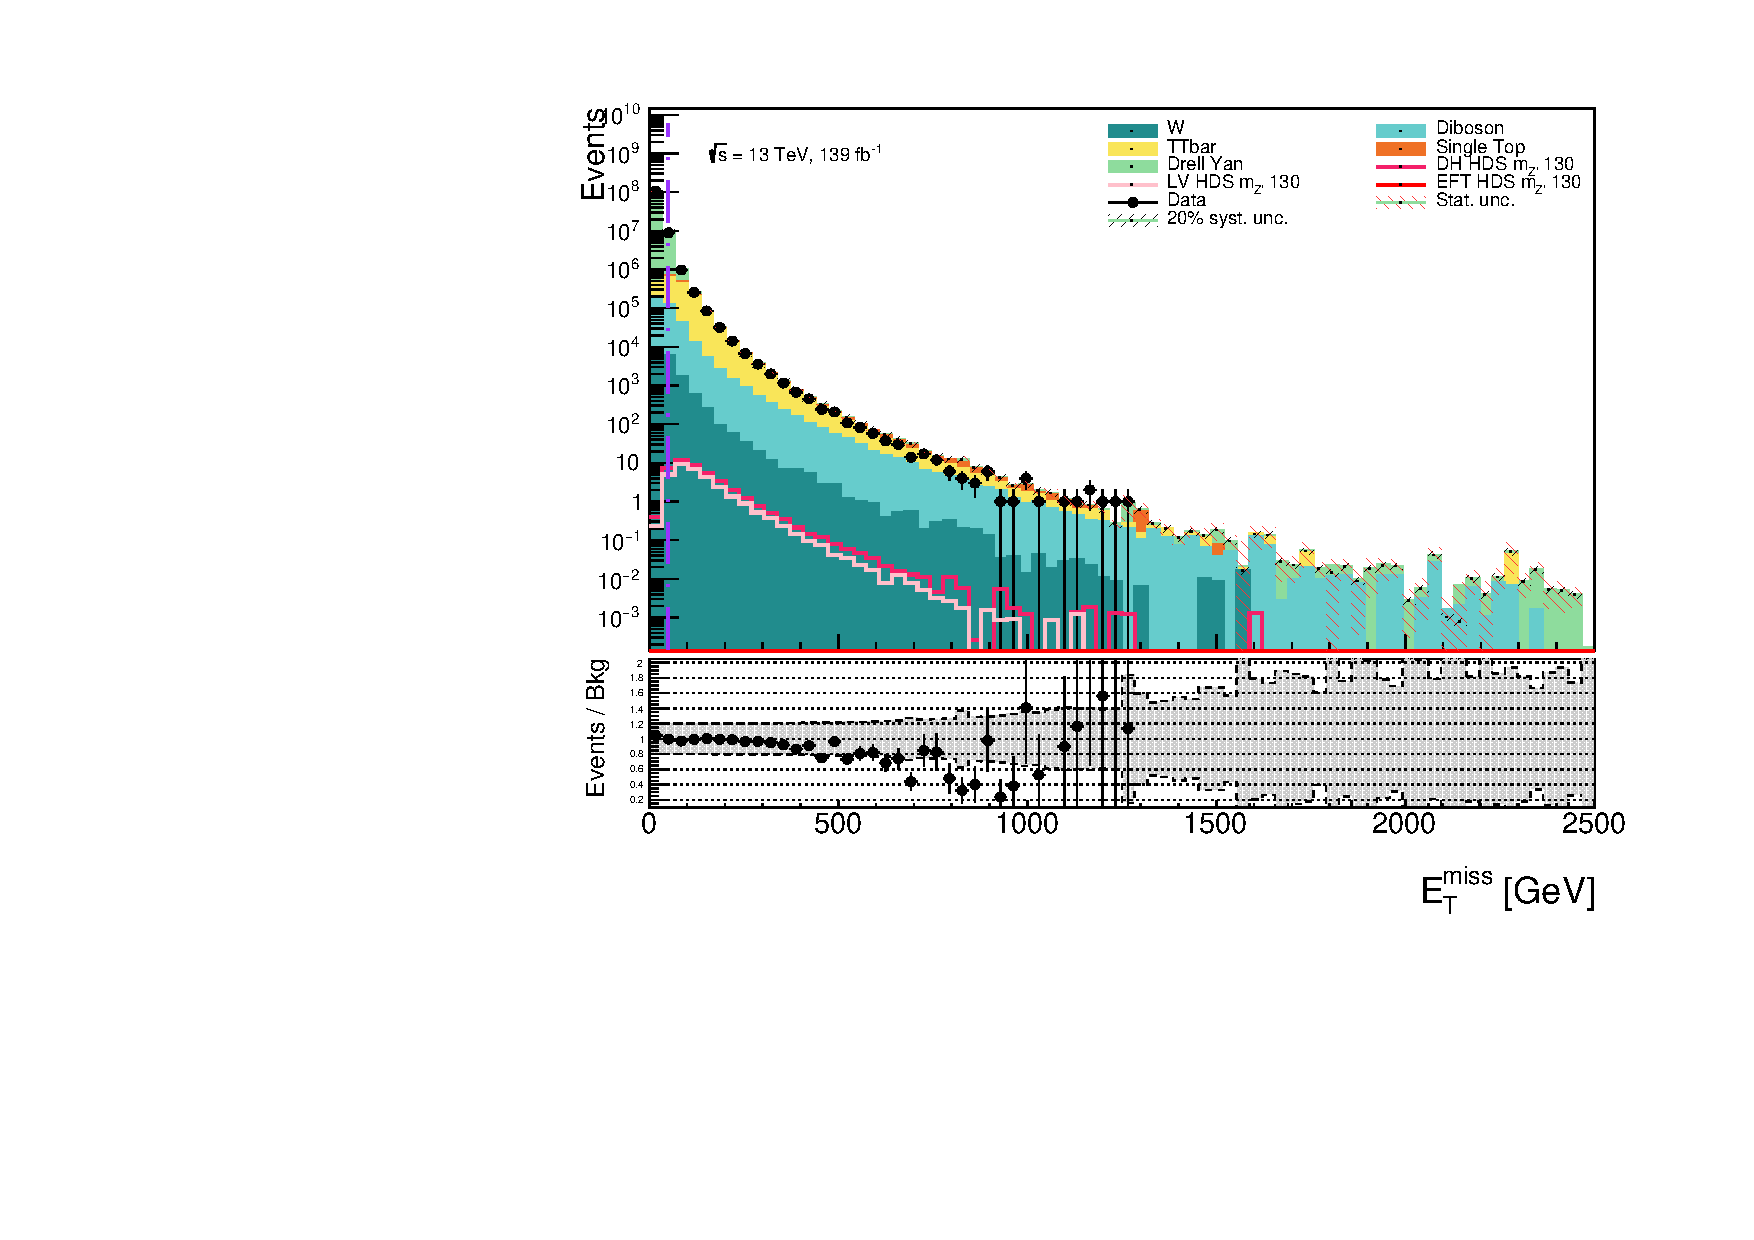
\includegraphics[width=0.8\textwidth]{met.pdf}
    \caption[$E_T^{miss}$ distribution in dilepton final state Run II]{Distribution of MET when looking at a dilepton final state in all of Run II. The violet line shows where we will make out MET cut to create a preselection region. The DM models here have the highest cross-section making them the most visible to our purposes.}\label{fig:uncut_met}
\end{figure}
\\Other than the object selection criteria, these are the only cuts that will be used to define the preselection region. Their summary can be seen in Table \ref{tab:CR_cuts}
\begin{table}[!h]
    \centering\caption[preselection region for model-independent search]{Table showcasing the cuts used to define the preselection region for our model independent search.}
    \begin{tabular}{l|r}\midrule\midrule
        Feature                                                                 & Selection criteria        \\\midrule
        Dilepton final state                                                    & $\ell^\pm \ell^\mp$, $\ell^\pm \ell^\pm$, $\ell^\pm \ell'^\mp$ and $\ell^\pm \ell'^\pm$    \\
        Missing Transverse Energy                                               & $E_T^{miss} > 50$ GeV     \\\midrule\midrule
    \end{tabular}
    \label{tab:CR_cuts}
\end{table}


\section{Feature selection for ML}
For this thesis there are many possible kinematic variables that can be used as features for our ML algorithms, in this section we will make use of the kinematical variables presented in Section \ref{sec:particle_kinematics} as well as introduce new variables that 
might help our ML algorithm to correctly learn the patters of SM background and DM signal events. \\
\\As we are studying a final state with two leptons it is natural to look at the kinematics for both of these objects. The first thing we will look at is the transverse momentum, $p_T$, of each lepton as defined in Eq. (\ref{eq:transverse_momentum}). 
We will also look at the azimuthal angle, $\phi$ and the pseudorapidity, $\eta$ defined in Eq. (\ref{eq:pseudorapidity}). 
With this we have practically constructed a four-momentum from which we could learn all particle kinematics. However, we want to help our ML algorithm as much as possible in the task of learning SM background and DM signal. A powerful kinematical variable for this is 
therefor the invariant mass, $m_{ll}$ defined in Eq. (\ref{eq:invariant_mass}), which can help the ML algorithm sort out resonant models. Another variable of interest is the transverse energy, $E_T$ defined in Eq. (\ref{eq:transverse_energy}) for the lepton pair. 
The distribution of the invariant mass can be seen in Figure \ref{fig:mll_dist}.\\
\graphicspath{{../../../Plots/Data_Analysis/SRs/Control_region/}} 
\begin{figure}[!ht]
    \centering
        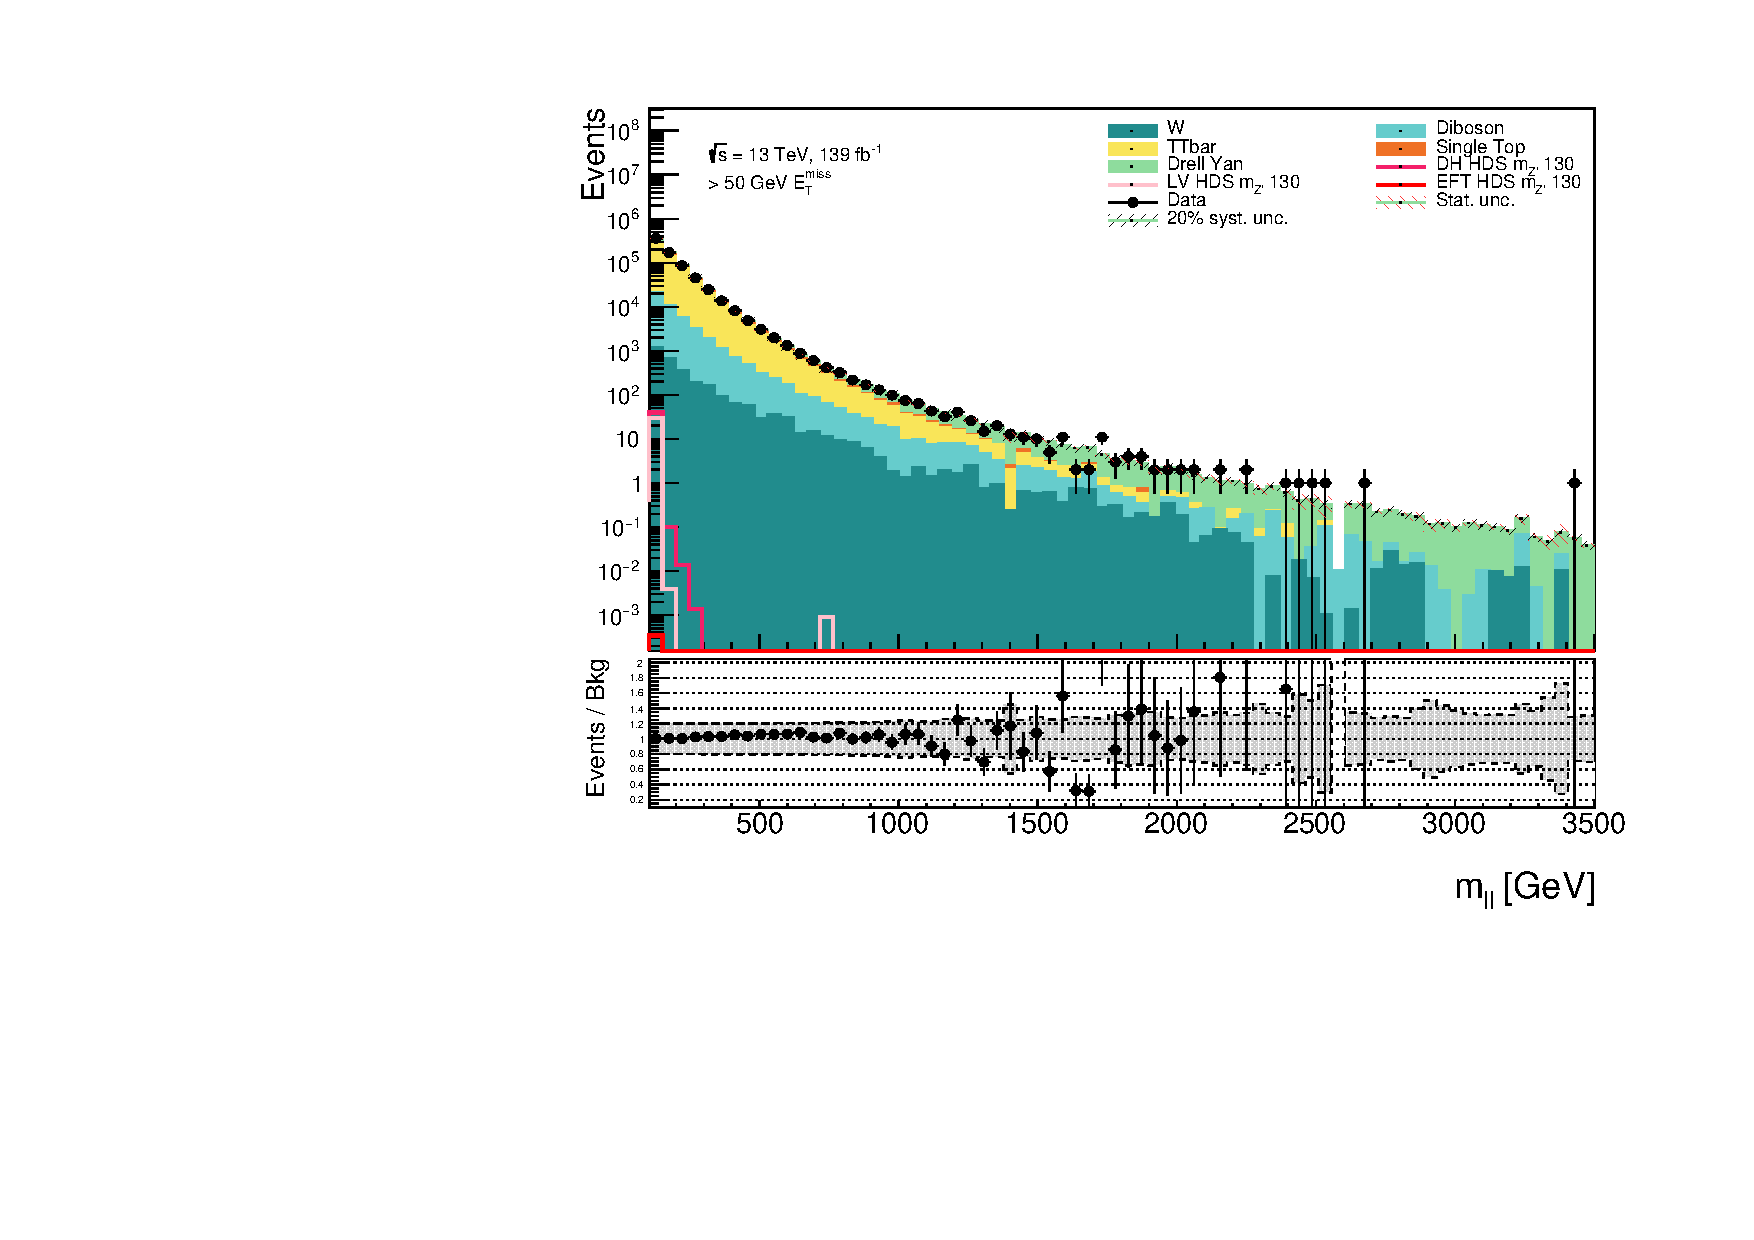
\includegraphics[width=0.8\textwidth]{mll.pdf}
    \caption{Distribution of $m_{ll}$ in preselection region.}\label{fig:mll_dist}
\end{figure}
\\As we are studying DM, an invisible particle, the most important kinematical variable to distinguish background from signal is the missing transverse energy, $E_T^{miss}$.
Another version of the MET is the so-called \textit{Object-based $E_T^{miss}$ significance}, or $E_T^{miss,sig}$ for short, this variable is used to deal with artificial or fake $E_T^{miss}$. The way $E_T^{miss,sig}$ works is by 
weighing the value of $E_T^{miss}$ by the precision of its reconstruction. It is defined as
\begin{equation}\label{eq:METsig}
    E_T^{miss,sig} = \frac{E_T^{miss}}{\sigma(E_T^{miss})}
\end{equation}
where $\sigma(E_T^{miss})$ is the uncertainty of the reconstruction of the $E_T^{miss}$, which consider the individual uncertainties of the objects that enter the $E_T^{miss}$ calculation. The distribution of this variable can ve seen in Figure \ref{fig:met_sig_dist}. 
In this thesis we will use both $E_T^{miss}$ and $E_T^{miss,sig}$ even though they are correlated, as the algorithm might choose in different instances\footnote{Meaning different \textit{signal regions} when conducting a model independent search. See Chapter \ref{sec:SRs}} 
which of these is of more importance.\\
\begin{figure}[!ht]
    \centering
        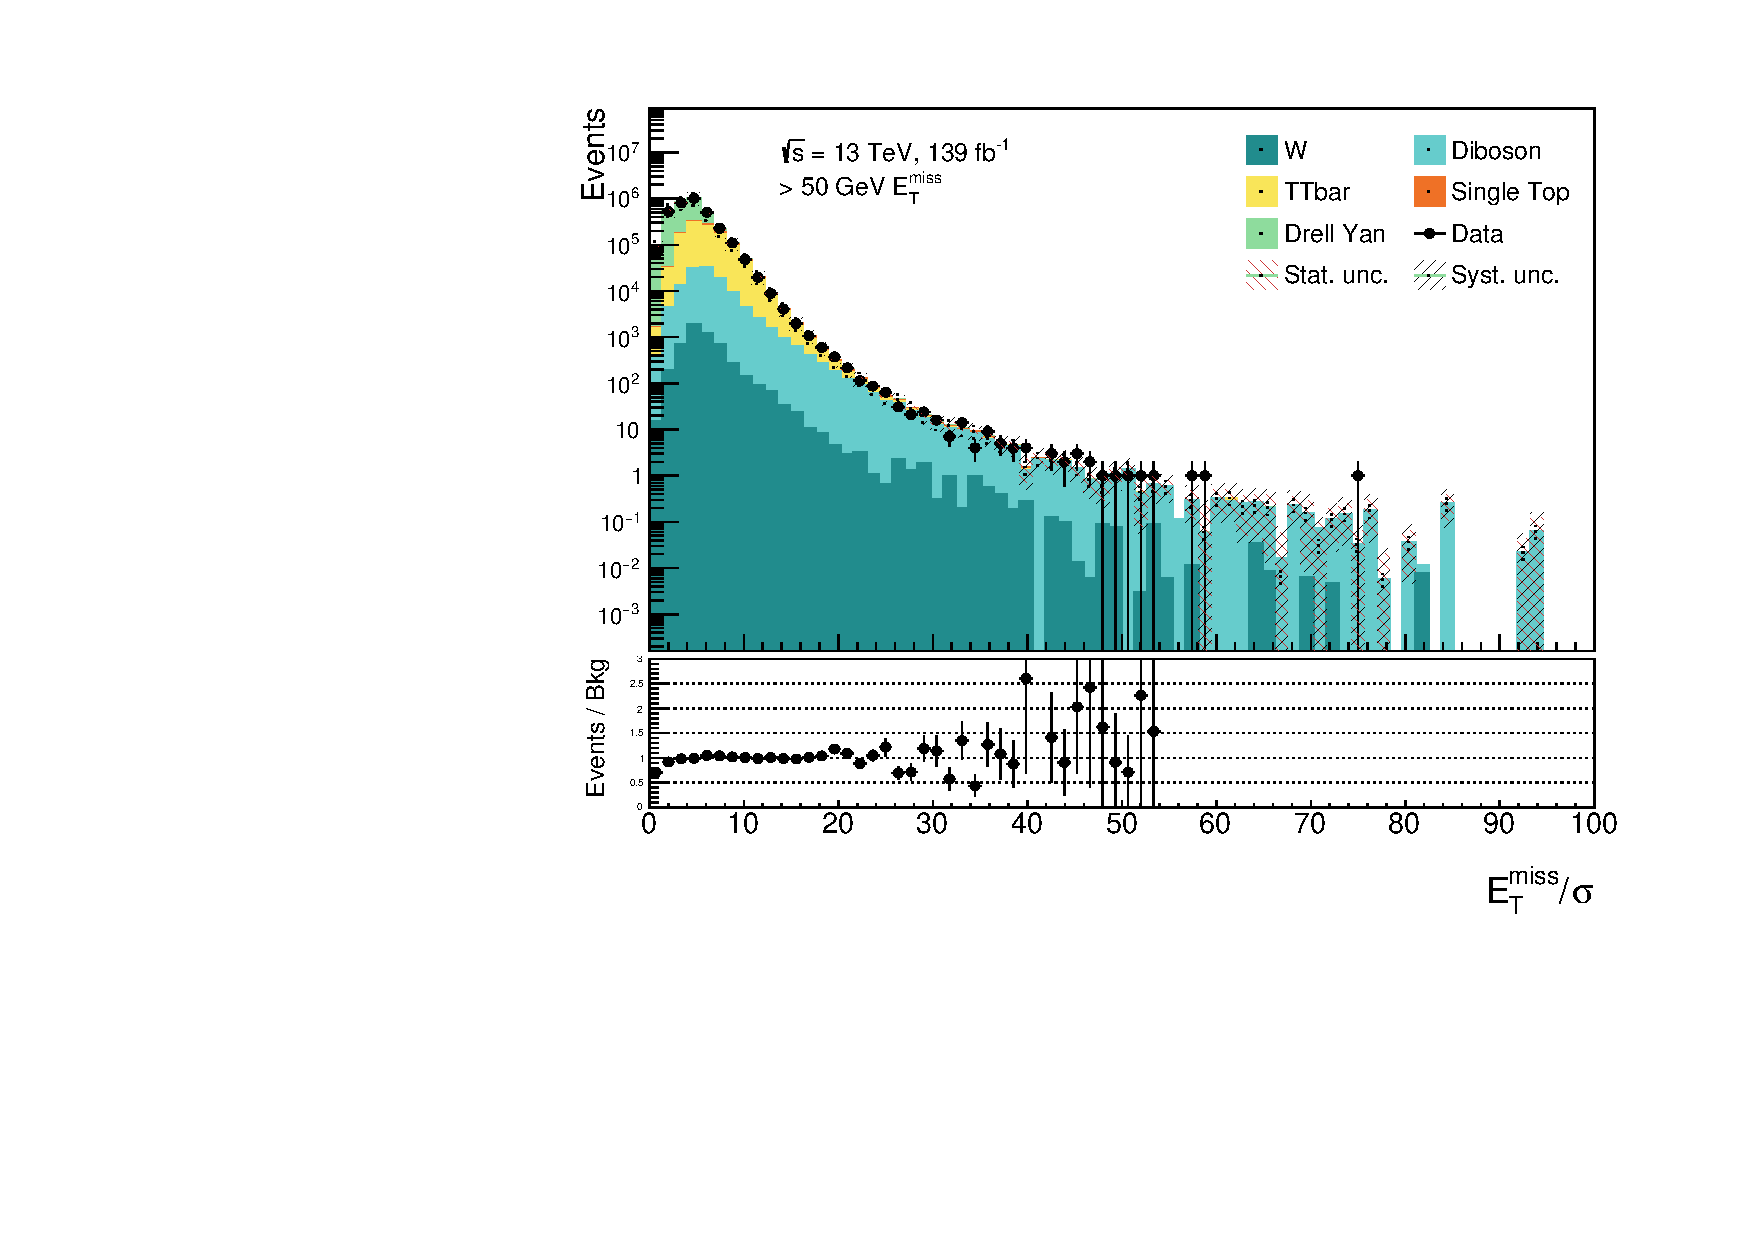
\includegraphics[width=0.8\textwidth]{met_sig.pdf}
    \caption{Distribution of $E_{T}^{miss,sig}$ in preselection region.}\label{fig:met_sig_dist}
\end{figure}
\\To keep the trend of variables for invisible particles, we will also study the transverse mass, $m_T$ defined in Eq. (\ref{eq:transverse_mass}), and stransverse mass, $m_{T2}$ defined in Eq. (\ref{eq:stransverse_mass}). 
The distribution of the stransverse mass can be seen in Figure \ref{fig:mt2_dist}. Moving on to jet related variables, we will count the number of b- and light jets with $p_T \ge 30, 40$ GeV respectively. As the jet reconstruction is already a hard task, 
which becomes even harder when pushing the limits of our selection criteria with a MET cut. In Appendix \ref{appendix:JetSelection} we can see how the data and MC simulations of the SM agree when counting the number of b- and light jets with a $p_T$ cut of $\ge30$ GeV and $\ge40$ GeV respectively. 
The agreement with different $p_T$ cuts can be seen in Appendix \ref{appendix:JetSelection}. We will also look at the $p_T$, $\eta$ and $\phi$ of the three most energetic jets, as these have the best MC and data agreement 
(see Figure \ref{fig:jetcuts}), and the invariant mass of the two most energetic jets $m_{jj}$.\\ 
\\Another variable we will look at is the hadronic activity, $H_T$ defined in Eq. (\ref{eq:HT}), from which we will also look at the ratio between the MET and hadronic activity, $E_T^{miss}/H_T$.\\
\begin{figure}[!ht]
    \centering
        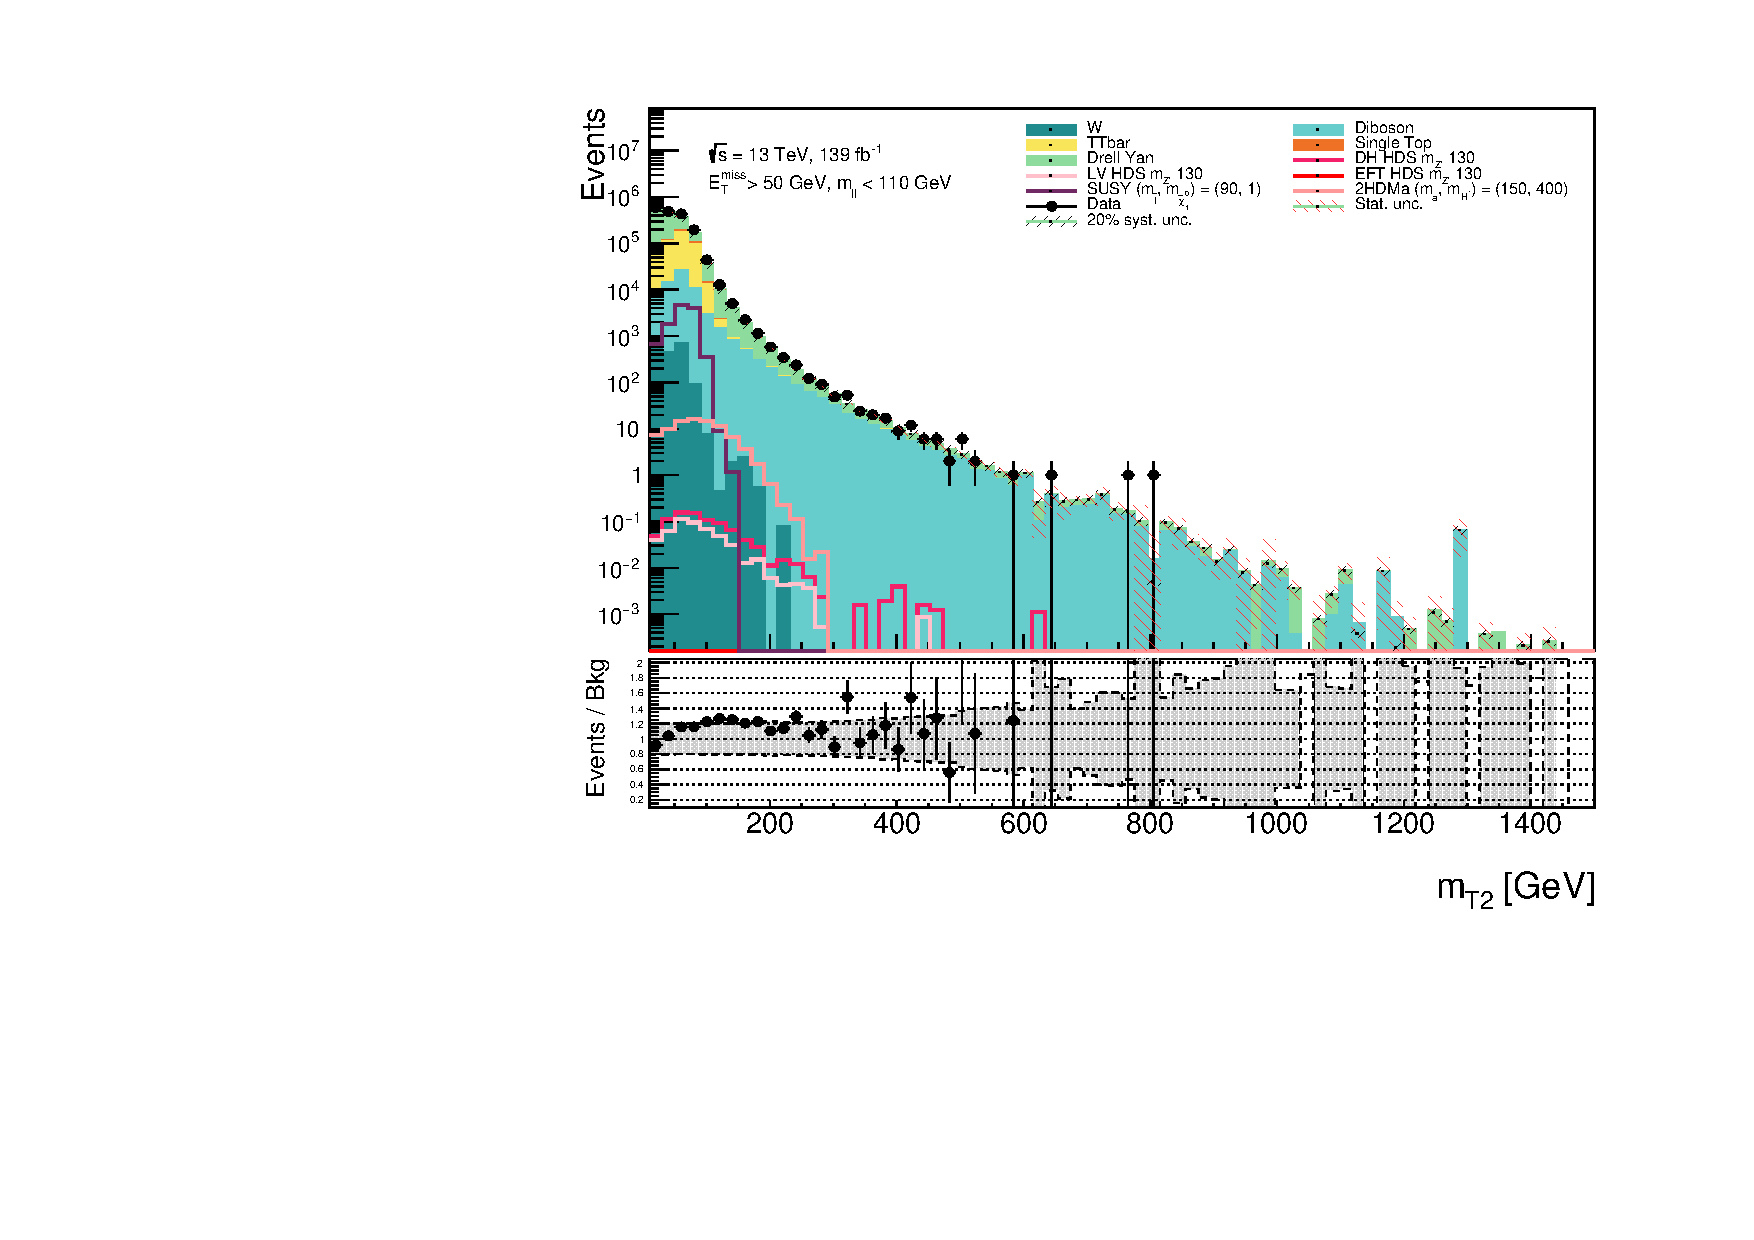
\includegraphics[width=0.8\textwidth]{mt2.pdf}
    \caption{Distribution of $m_{T2}$ in preselection region.}\label{fig:mt2_dist}
\end{figure}
% \graphicspath{{../../../Plots/Data_Analysis/JetSelection/Control_region/}} 
% \begin{figure}[!ht]
%     \centering
%     \hfill\begin{subfigure}[b]{0.49\textwidth}
%         \centering
%         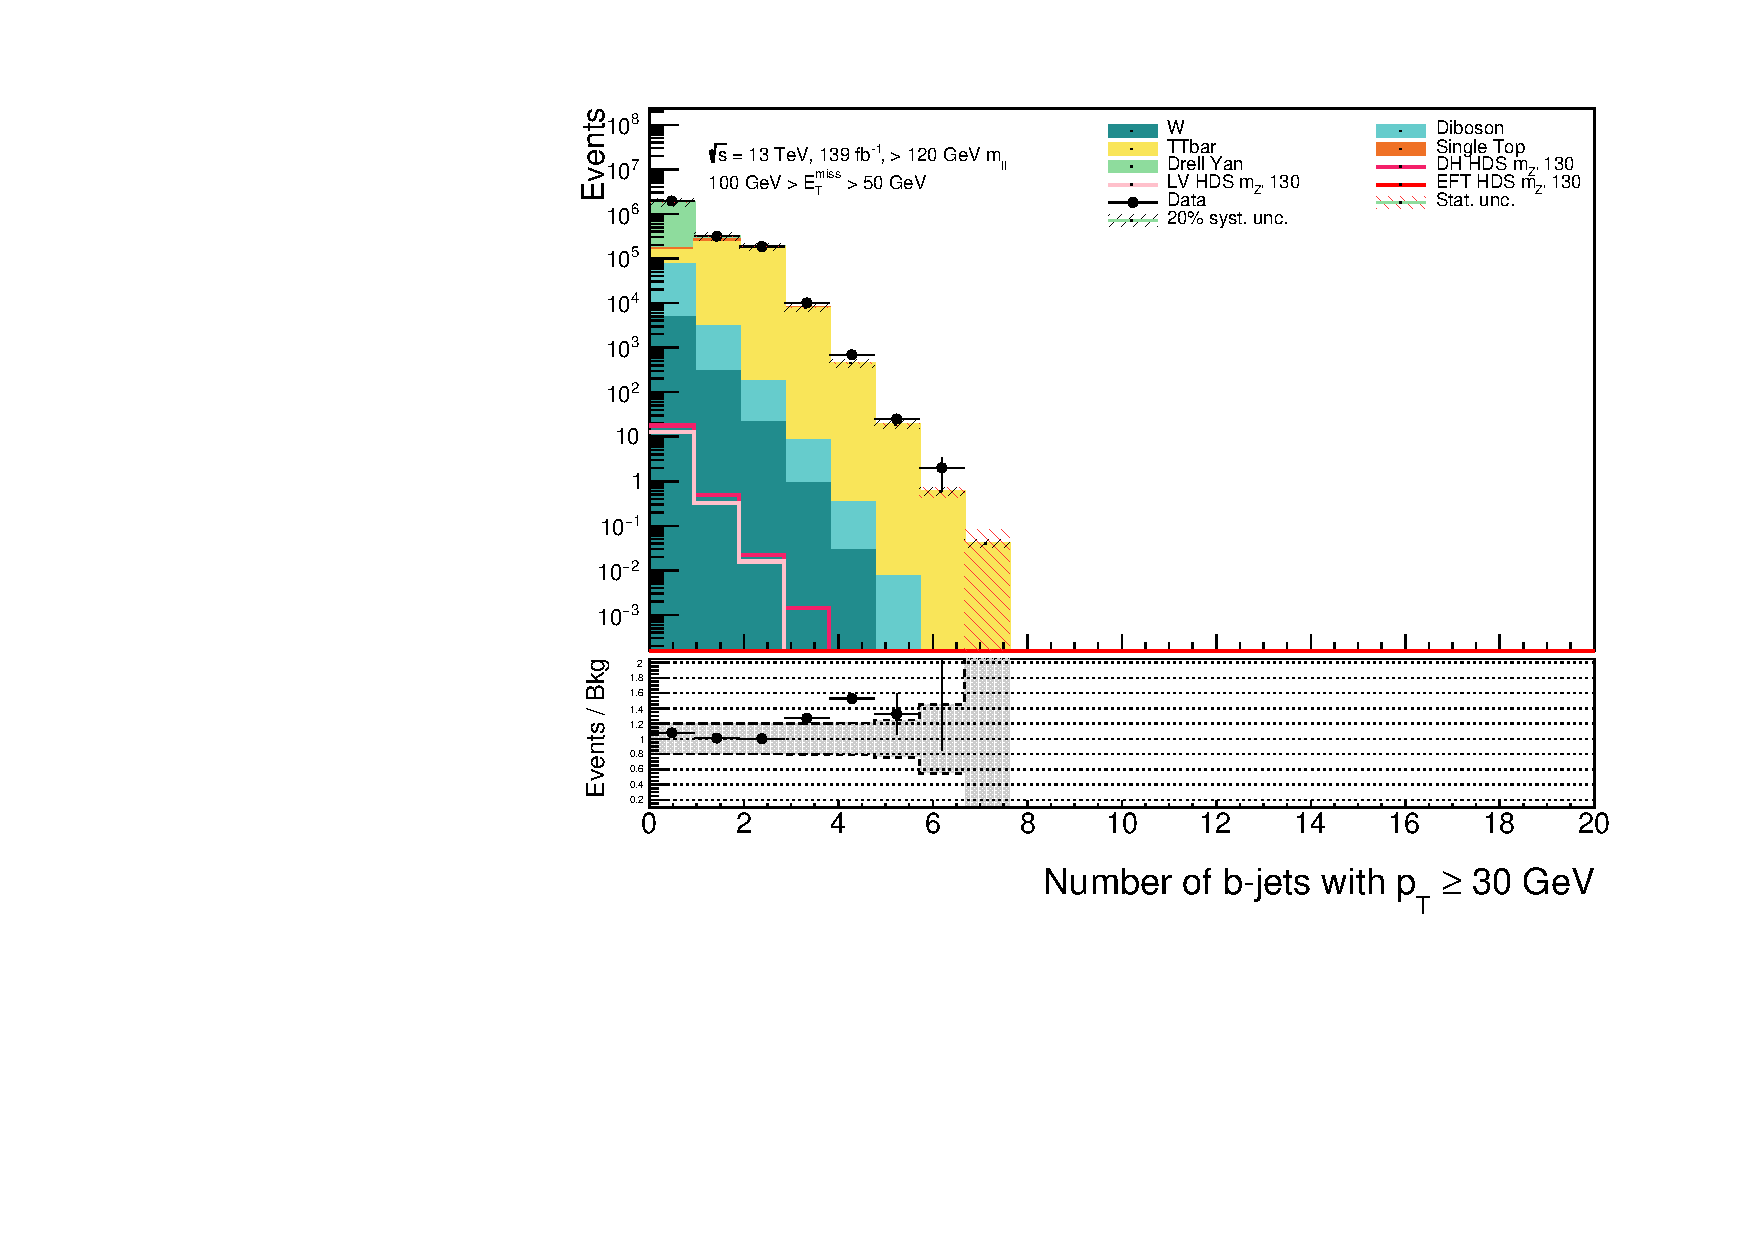
\includegraphics[width=\textwidth]{bjetsPt30.pdf}
%     \end{subfigure}
%     \hfill\begin{subfigure}[b]{0.49\textwidth}
%         \centering
%         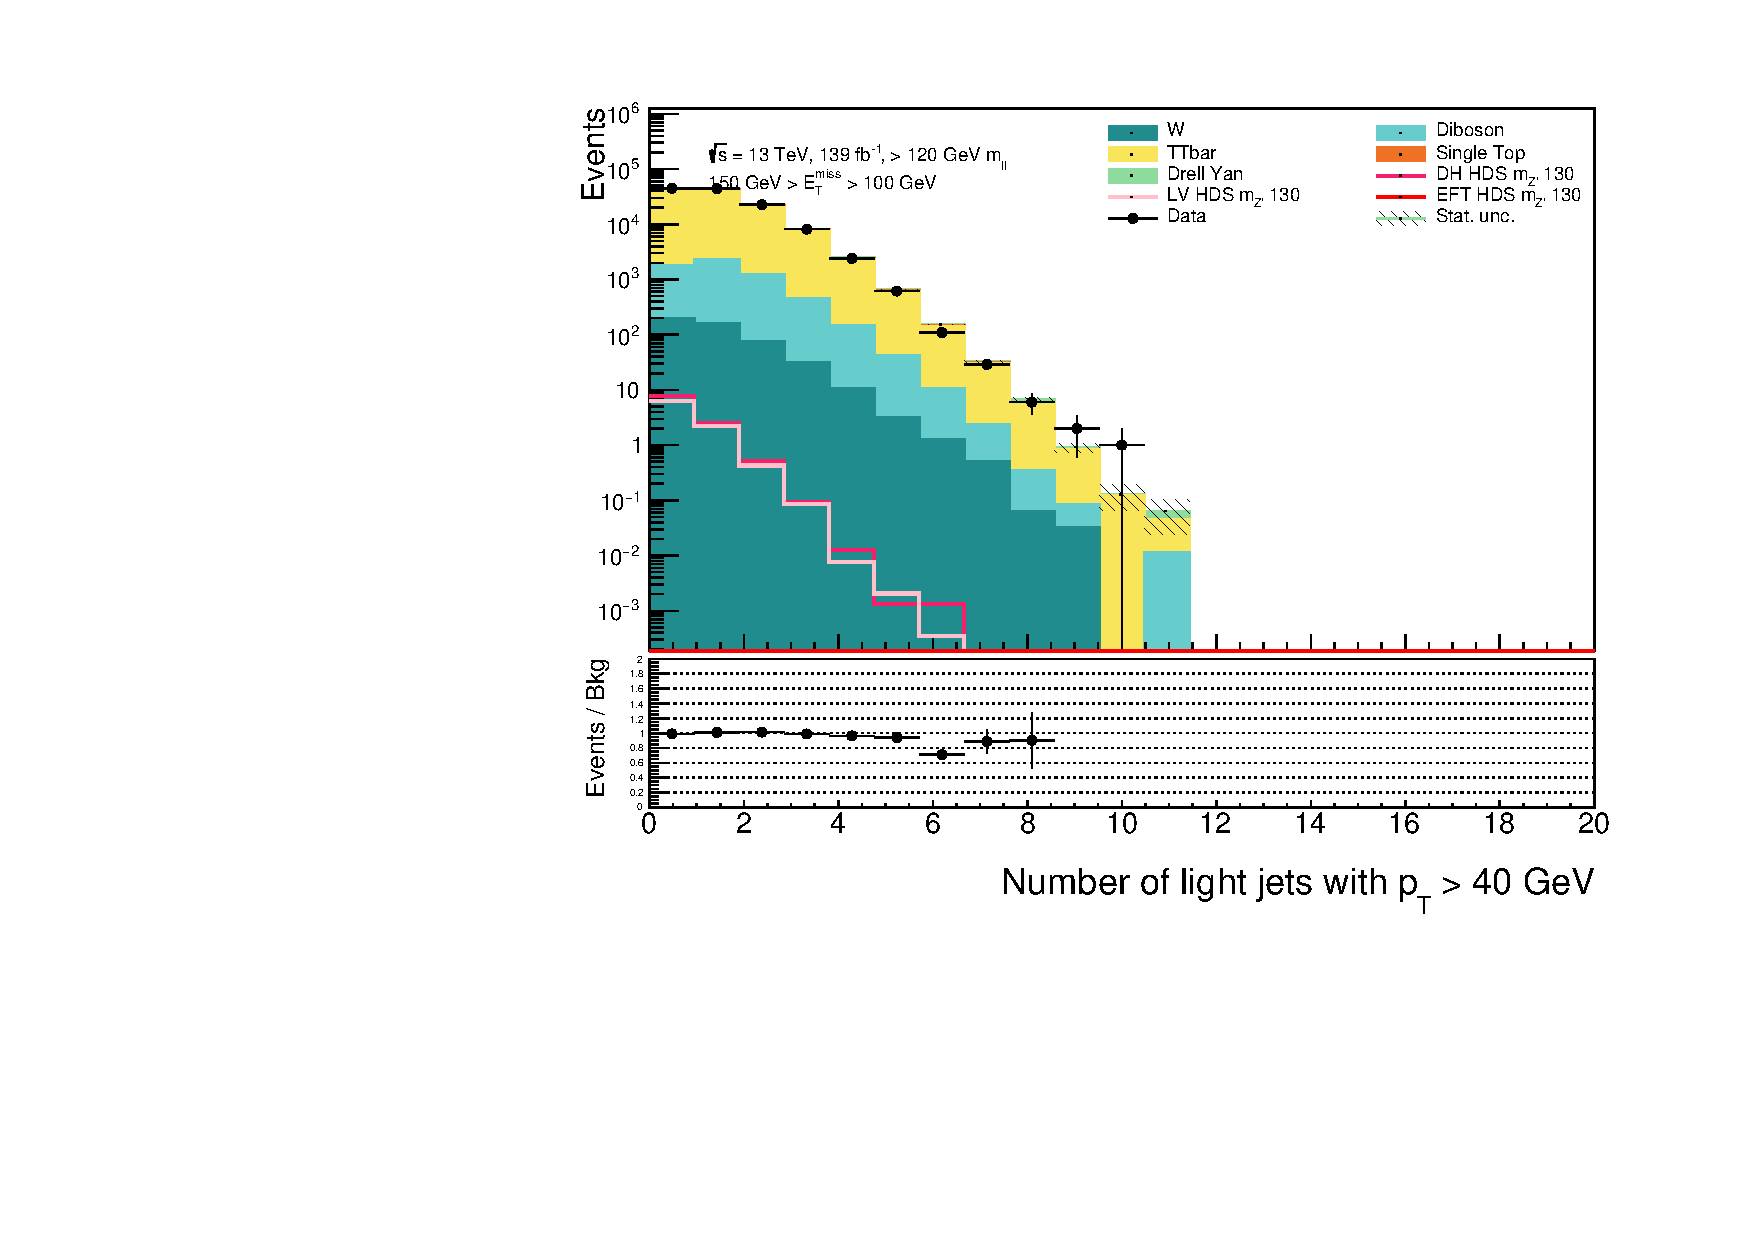
\includegraphics[width=\textwidth]{ljetsPt40.pdf}
%     \end{subfigure}
%     \caption[b- and light jet distributions in preselection region]{b- and light jet distributions with $p_T \ge30$ and $\ge40$ GeV, respectively.}\label{fig:jetcuts}
% \end{figure}
\graphicspath{{../../../Plots/Data_Analysis/SRs/Control_region/}} 
\\To know the distance between the lepton and MET we will look at the difference in azimuthal angle between: the lepton pair, $\Delta\phi(l_1,l_2)$, the dilepton system and MET, $\Delta\phi(ll,E_T^{miss})$, the leading lepton and MET, $\Delta\phi(l_l,E_T^{miss})$, 
and the lepton closest to the MET and the MET, $\Delta\phi(l_c,E_T^{miss})$. In some of the models we are studying it is expected for DM and the lepton pair to be back to back. The distribution of $\Delta\phi(ll,E_T^{miss})$ can be seen in Figure \ref{fig:dPhiLLMET_dist}.
\begin{figure}[!ht]
    \centering
        \includegraphics[width=0.8\textwidth]{dPhiLLMET.pdf}
    \caption{Distribution of $\Delta\phi(ll,E_T^{miss})$ in preselection region.}\label{fig:dPhiLLMET_dist}
\end{figure}

\clearpage\noindent The kinematic variables used are summarized in Table \ref{tab:variables} and the distribution of the remaining kinematical variables are shown in Appendix \ref{apendix:Kin_var_in_CR}.
\begin{table}[!h]
    \centering
    \caption[Kinematic variables used as features]{Table showcasing the kinematic variables that will be used as features on our ML algorithm.\\ * These have poor MC and data agreement. $^\dagger$ These create \textit{jagged arrays}.}
    \begin{tabular}{l|r}\midrule\midrule
        Kinematic variable                                                              & Feature name          \\\midrule
        $p_T$ of both leptons                                                           & lep1pt \& lep2pt      \\
        $\phi$ of both leptons                                                          & lep1phi \& lep2phi    \\
        $\eta$ of both leptons                                                          & lep1eta \& lep2eta    \\
        Invariant mass of dilepton pair, $m_{ll}$                                       & mll \\
        Missing transverse energy in event, $E_T^{miss}$                                & met \\
        Missing transverse energy significance in event, $E_T^{miss,sig}$               & met\_sig \\
        Transverse mass in an event, $m_T$                                              & mt \\
        Stransverse mass in an event, $m_{T2}$                                          & mt2\\
        Transverse energy of lepton pair, $E_T$                                         & et \\
        $\phi$ between lepton pair, $\Delta\phi(l_1,l_2)$*                              & dPhiLeps \\
        $\phi$ between lepton pair and MET jet, $\Delta\phi(ll,E_T^{miss})$             & dPhiLLMet \\
        $\phi$ between leading lepton and MET jet, $\Delta\phi(l_l,E_T^{miss})$         & dPhiLeadMet \\
        $\phi$ between the closest lepton and MET jet, $\Delta\phi(l_c,E_T^{miss})$*    & dPhiCloseMet \\
        Hadronic activity, $H_T$                                                        & ht\\
        Ratio between $E_T^{miss}$ and $H_T$, $E_T^{miss}/H_T$                          & rt\\
        Number of b-jets                                                                & nbjets         \\
        Number of light jets*                                                           & nljets         \\
        $p_T$ of three jets with highest $p_T$$^\dagger$                                & jet1pt \& jet2pt \& jet3pt\\
        $\phi$ of three jets with highest $p_T$$^\dagger$                               & jet1phi \& jet2phi \& jet3phi\\
        $\eta$ of three jets with highest $p_T$$^\dagger$                               & jet1eta \& jet2eta \& jet3eta\\
        Invariant mass of two jets with highest $p_T$, $m_{jj}$$^\dagger$               & mjj\\\midrule\midrule
    \end{tabular}
    \label{tab:variables}
\end{table}

\subsection{MC and data disagreement} 
There is a challenge, with the final states that are not SFOS, as the MC generated background on these tend to be lower than the recorded data. The number of events that are not SFOS are minimal though, 
and we think the reason it does not fit the data is because we are not including fake leptons. The features where these are prominent are marked by a * on Table \ref{tab:variables}.

\section{Transfer to ML friendly syntax}
We have so far explained how the data will be used and carefully selected, however the question of how the data is made, and the number of samples we will work with still remains unanswered. \\
\\The MC simulations are made into \verb|ROOT| \cite{ROOT} NTuples which contain the information of the objects passing our selection criteria in each event. What remains is to set the kinematical cuts, so we have our preselection region. 
To do this as well as saving the remaining events into a new file which will be used for our ML algorithm I utilized the algorithms on \verb|EventSelector|\footnote{Available here: \href{https://github.com/rubenguevara/Master-Thesis/tree/master/EventSelector}{https://github.com/rubenguevara/Master-Thesis/tree/master/EventSelector}}, 
which also saved the events that passed the event selection criteria as \verb|ROOT| histograms to make plotting the distributions easier. After saving the events that passed the selection criteria I used the algorithms on \verb|DataPrep|\footnote{Available here: \href{https://github.com/rubenguevara/Master-Thesis/tree/master/DataPrep}{https://github.com/rubenguevara/Master-Thesis/tree/master/DataPrep}} 
to plot the actual distributions of kinematical variables, and more importantly converting all the events that passed the event selection into an ML friendly syntax. For this thesis we are converting from \verb|ROOT| NTuples to \verb|pandas DataFrame| \cite{pd.DataFrame} 
which can furthermore be saved as \verb|h5| files to be read more efficiently. The reason we chose \verb|pandas DataFrame| is because of the easily readable kinematics per event, the easily applicable kinematical cuts to the whole dataset 
(to more effectively create signal regions), and most importantly because of the compatibility with \verb|XGBoost| \cite{XGBoost} and \verb|TensorFlow| \cite{TensorFlow} which will be the ML packages we will utilize for both BDTs and NNs. 
With this we are ready to discuss the preparation of our ML algorithms.

% \section{Additional data preparation needed for ML application}
% There are however still challenges that needs to be addressed before starting our ML, the biggest are addressed here.
% \\Now that we have explained how the data has been prepared and the problems that arise with this we are ready to start playing around with ML!
% \textbf{Question: Anything else to add to this chapter?}



\end{document}